\documentclass[12pt]{article}
\usepackage{sbc-template}
\usepackage{graphicx,url}
\usepackage{float}
\usepackage[brazil]{babel}   
\usepackage[utf8]{inputenc}  
\usepackage{url}
\bibliographystyle{ieeetr}

\usepackage{inconsolata}

\usepackage{color}

\definecolor{pblue}{rgb}{0.13,0.13,1}
\definecolor{pgreen}{rgb}{0,0.5,0}
\definecolor{pred}{rgb}{0.9,0,0}
\definecolor{pgrey}{rgb}{0.46,0.45,0.48}

\usepackage{listings}
\lstset{language=Java,
	showspaces=false,
	showtabs=false,
	breaklines=true,
	showstringspaces=false,
	breakatwhitespace=true,
	commentstyle=\color{pgreen},
	keywordstyle=\color{pblue},
	stringstyle=\color{pred},
	basicstyle=\ttfamily
}
     

\sloppy
	\title{ Simulação de Pool de Impressão Dístribuida Utilizando Socket \\ Exercício Computacional II - Sistemas Distribuídos}

\author{Rafael Gonçalves de Oliveira Viana\inst{1}  }


\address{Sistemas de Informação -- Universidade Federal do Mato Grosso do Sul
	(UFMS)\\
  	Caixa Postal 79400-000 -- Coxim -- MS -- Brazil
  \email{rafael.viana@aluno.ufms.br }
  \\\vspace*{10pt} \normalsize  \today{}
}

\begin{document} 

\maketitle

     
\begin{resumo} 	
  Este  documento relata como foi o desenvolvimento de uma Pool de Impressão na linguaguem Java versão 8, utilizando Threads e Sockets.
\end{resumo}

\section{Introdução}
De acordo com \cite{entf}, em um ambiente de trabalho, onde desejasse imprimir documentos enviados, a um curto período de tempo, é necessário a utilização de uma pool de impressão.

Uma pool de impressão permite que várias impressoras físicas possam ser controladas por uma única impressora lógica,  sempre que um trabalho for enviado para a impressora lógica, está consultará o estado das impressoras físicas para verificar qual equipamento está livre no momento e enviará o trabalho para ela.
 Um exemplo de pool de impressão é demonstrada na figura \ref{fig:screenshot001}.

\begin{figure}[H]
 	\centering
 	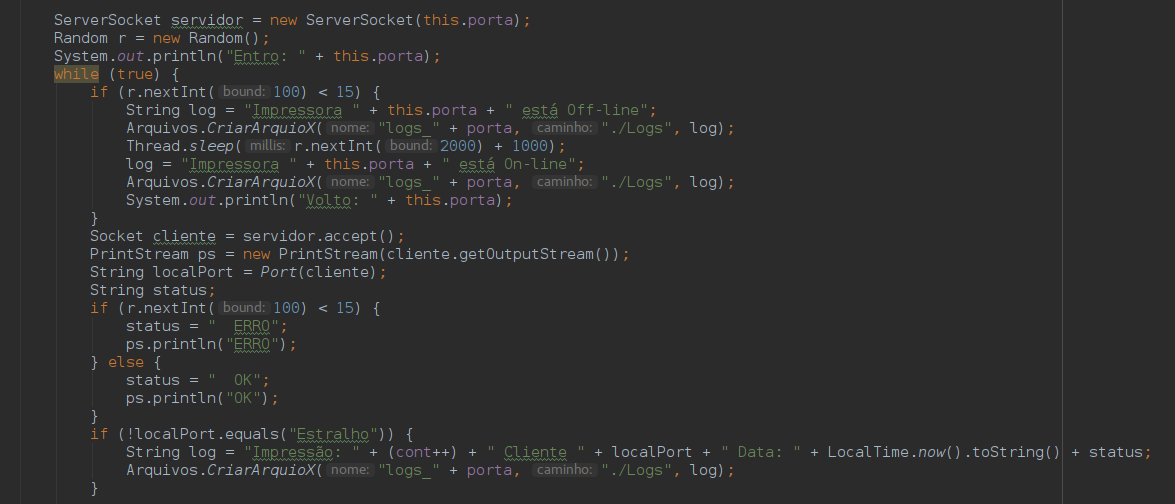
\includegraphics[width=0.7\linewidth]{imagens/screenshot001}
 	\caption{Proposta do exercício computacional.}
 	\label{fig:screenshot001}
 \end{figure}
 
\section{Fundamentação Téorica} 
	Nesta seção serão tratadas, soluçoes de problemas pertinentes que foram utilizadas neste documento.


\subsection{Problema de Concorrência}
O problema de concorrência existem em diversos cenários em que, um pedaço de código que definimos como crítico não pode ser executado por duas threads ou mais, ao mesmo tempo. Apenas uma thread por vez consegue entrar em alguma região crítica e realizar determina função.

	O java realiza a syncronyzação das threasd
	
	Para mais informações referente a sincronização de threads na linguagem java consultar a referência \cite{ct}.

 
\subsection{Socket}

 Segundo \cite{socket}.\cite{conc}.
 Os sockets são compostos por um conjunto de primitivas do sistema operacional e foram originalmente desenvolvidos para o BSD Unix. Sockets são suportados em Java desde o JDK 1.0, para sua utilização devemos fazer uso das classes contidas no pacote java.net.\ref{fluxoSocket}.
\begin{figure}[H]
	\centering
	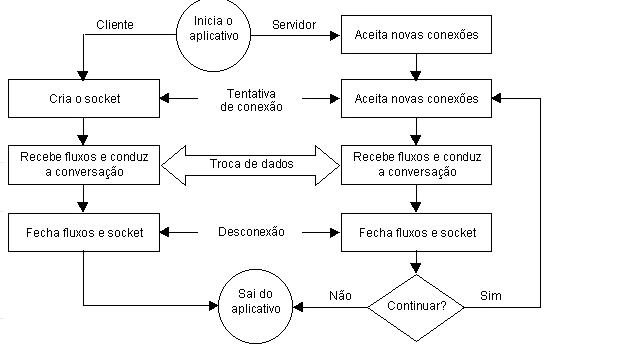
\includegraphics[scale=1]{imagens/fluxoSocket.JPG}
    \caption{Fluxo de troca de dados com sockets.}
	\label{fluxoSocket}
\end{figure}

 \subsection{Problema de Espera Ocupada} \label{Espera}
 	
 Para mais informações referente a espera ocupada de threads na linguagem java consultar as referências \cite{conc} \cite{wait}.
\section{Desenvolvimento}
Para resolver o trabalho proposto, foi desenvolvido uma aplicação java que simula, uma pool de impressões que as ordena e envia para uma impressora.
Foram criadas 3 classes Javas sendo elas: Cliente , Pool de Impressão e Impressora.
As mesmas serão comentadas nas próximas seções.
\subsection{Cliente}
	Essa classe  se conecta a classe servidor, repassando informações via Socket, em uma via de mão dupla.
Os dados serão aceitos na memória e posteriormente serão alocados no pelo escalonador da pool de impressão, em alguma impressora disponível, onde mais tarde será notificado com o resultado da processamento da impressão.

O código responsável pela chamada de impressão no cliente e simples, podemos observar o método na figura  \ref{fig:screenshot005}.

\begin{figure}[H]
	\centering
	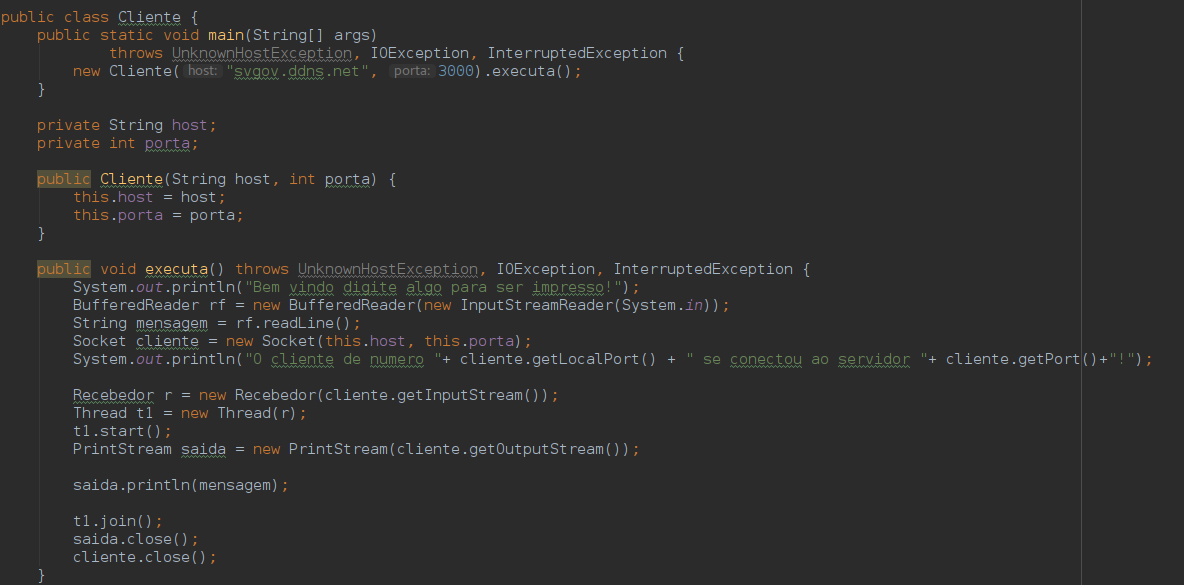
\includegraphics[width=1\linewidth]{imagens/screenshot005}
	\caption{Código cliente, da pool de impressão.}
	\label{fig:screenshot005}
\end{figure}



\subsection{Pool de Impressão - Servidor}\label{pool}
  Classe responsável pela comunicação dos Sockets (Cliente/Impressora), ela contém o escalonador  de impressão, que  é responsável por designar os serviços na pool de impressão.
  
	  O código do servidor é responsável por 3 threads sendo elas:
	  \begin{enumerate}
	  	\item Aceitar conexões via Socket e adicionar documento para impressão.
	  	\item Procurar impressoras disponíveis (escalonador de impressão)
	  	\item Enviar documento para impressoras e receber resposta de confirmação das mesmas.
	  \end{enumerate}
	
	A figura \ref{fig:screenshot006} demonstra a função que inicializa as variáveis proposta no exercício computacional, além de iniciar as Threads do servidor. 
O responsável por determinar quais impressoras estão disponíveis, e alocar trabalho para as mesmas, é o escalonador de impressão que é desenvolvido na classe \textit{Chegada de Documento}.
O escalonador ao perceber que não tem tarefas a realizar vai dormir wait(), quando um processo chega para ser escalonado ele acorda e realiza o repasse para a primeira impressora disponível, e volta a dormi.


\begin{figure}[H]
	\centering
	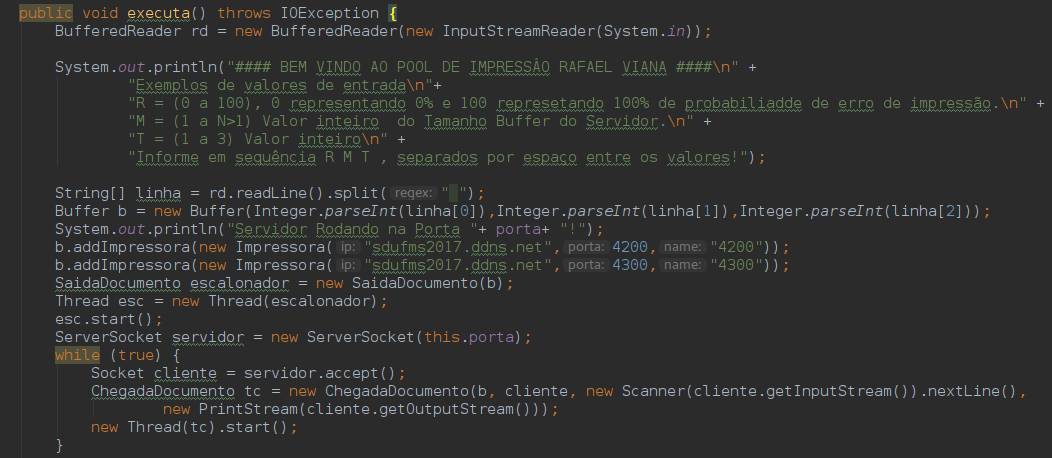
\includegraphics[width=1\linewidth]{imagens/screenshot017}
	\caption{}
	\label{fig:screenshot006}
\end{figure}
O código completo, incluindo todas as classes como na figura \ref{fig:screenshot008}, estão disponíveis no link https://github.com/rafaelgov95/SD/tree/master/PTJI/Projeto-PTJ


\begin{figure}[H]
	\centering
	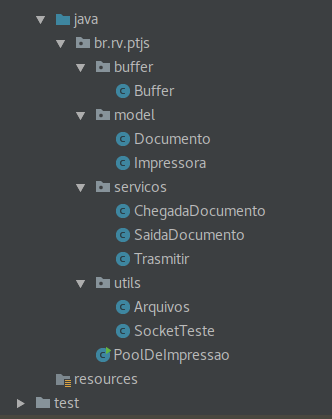
\includegraphics[width=0.4\linewidth]{imagens/screenshot016}
	\caption{Classes do Servidor de pool de Impressão}
	\label{fig:screenshot008}
\end{figure}



\subsection{Impressoras}\label{impre}
Classe responsável pela impressão dos documentos contidos  no buffer da Pool de Impressão \ref{pool}.

Ela trabalha junto ao escalonador do servidor, que é responsável por notificar as impressoras cadastradas, que novas impressões devem ser executadas, vale destacar que o escalonador foi desenvolvido, de acordo com a boa prática de não deixar uma espera ocupada.

A figura \ref{fig:screenshot002}, apresenta o método que realiza a criação das Threads.
Elas executam em modo servidor aguardando o escalonador alocar alguma tarefa.
\begin{figure}[H]
	\centering
	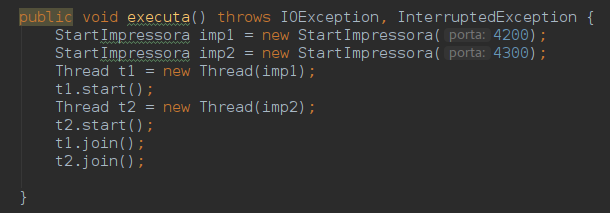
\includegraphics[width=1\linewidth]{imagens/screenshot002}
	\caption{Criação de duas impressoras pelo método StartImpressora.}
	\label{fig:screenshot002}
\end{figure}

Após a criação, as Threads que representam as impressoras, as mesmas ficam aguardando no while(true), que não gera espera ocupada, por causa do método de servidor, \textit{servidor.accept}, como na figura  \ref{fig:screenshot003}.
\begin{figure}[H]
	\centering
	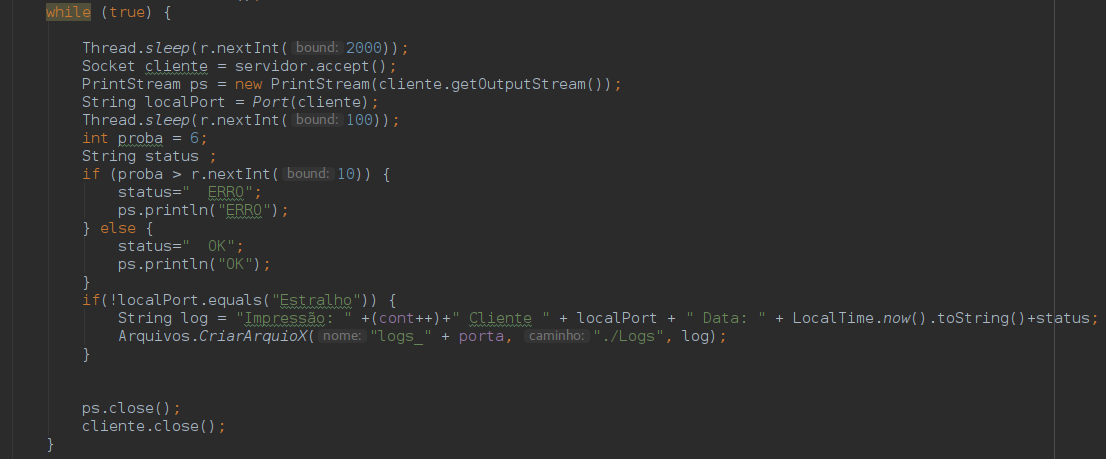
\includegraphics[width=1\linewidth]{imagens/screenshot003}
	\caption{}
	\label{fig:screenshot003}
\end{figure}
\section{Comandos da Implementação }
	Nesta seção será apresnetado os comandos para poder utilizar o Pool de Impressão. 
 
	\subsection{Cliente}
	
	\subsection{Servidor}
	
	\subsection{Impressoras}
 
 \section{Testes e Resultados }
 Nesta seção será demonstrado os logs das impressoras e do servidor após a conexão de 4 clientes, com o servidor.
 Para realizar os testes foram utilizado um Raspberry Pi3 e uma Virtual Machine da Google Developers.
 \subsubsection{Distribuição de Recursos}
 \begin{enumerate}
 	
 	\item Como servidor da pool de impressão ficou o Raspberry Pi3, demonstrando que a classe Servidor não precisa de um grande poder computacional para ser executada \ref{pool}.
 	\item Como impressoras virtuais da pool de impressão, que se encontra no Raspberry Pi3, foi utilizado uma Virtual Machine da Google Developer, com o código de impressoras virtuais.\ref{impre}
 \end{enumerate}

 \subsubsection{Passos}
 \begin{enumerate}

\item Primeiramente a requisição de algum cliente se conecta ao pool de impressão, presente no Raspberry Pi3, por meio do Socket.

\item Ao receber a requisição de impressão, a pool adiciona o documento ao Buffer, e acorda o escalonador de impressão que envia a impressão para, alguma impressora disponível na virtual machine da Google developers.

\item Ao receber o documento a impressora responde um "OK" para o pool, porém ela pode perder o documento e então envia uma mensagem de ERRO, o que provocaria o reenvio da mesma, até que consiga realizar a impressão.

\item Durante todos esses passos mensagens como "Adicionada à Fila" ou mensagens de erros, são encaminhadas para os clientes em tempo real.

\end{enumerate}
Agora que já entendemos como funciona a comunicação, podemos visualizar os relatórios, comecaremos pelo do escalonador, que após a execução dos 4 clientes é demonstrado na figura \ref{fig:screenshot009}.


 \begin{figure}[H]
 	\centering
 	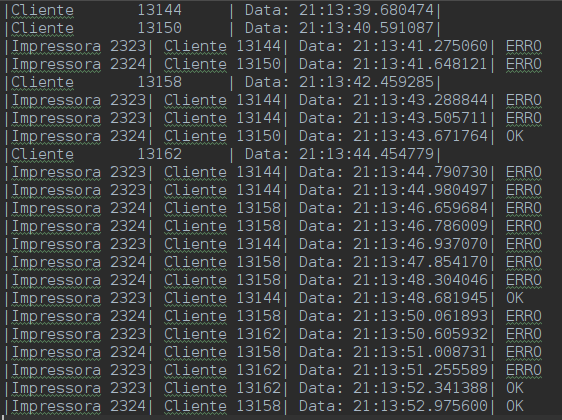
\includegraphics[width=0.7\linewidth]{imagens/screenshot014}
 	\caption{Relatório de impressões, registrado pelo escalonador presente no servidor.}
 	\label{fig:screenshot009}
 \end{figure}

 
 O relatório da impressora 4200, pode ser observado na figura \ref{fig:screenshot010}.

 \begin{figure}[H]
 	\centering
 	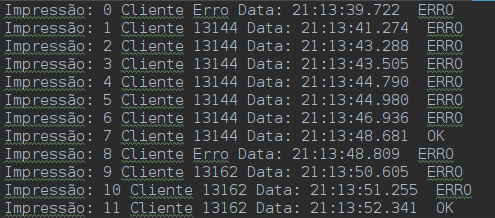
\includegraphics[width=0.7\linewidth]{imagens/screenshot013}
 	\caption{Relatório da impressora 4200, após execução dos 4 clientes.}
 	\label{fig:screenshot010}
 \end{figure}
 
  O relatório da impressora 4300, pode ser observado na figura \ref{fig:screenshot012}.
  \begin{figure}[H]
  	\centering
  	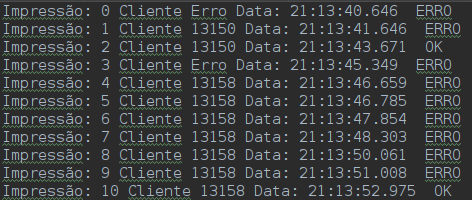
\includegraphics[width=0.7\linewidth]{imagens/screenshot012}
  	\caption{Relatório da impressora 4300, após execução dos 4 clientes.}
  	\label{fig:screenshot012}
  \end{figure}
  
  O cliente após  o envio do documento, aguarda a impressão do mesmo, enquanto isso recebe notificações  a respeito de sua impressão em tempo real, podemos ver  na figura  \ref{fig:screenshot015}, o resultado final de notificações do cliente.
  
  \begin{figure}[H]
  	\centering
  	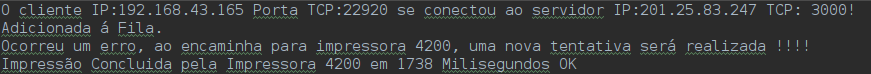
\includegraphics[width=0.7\linewidth]{imagens/screenshot015}
  	\caption{Notificações em tempo real de impressão para o Cliente.}
  	\label{fig:screenshot015}
  \end{figure}
  
\section{Conclusão}

Neste relatório foi demonstrado o desenvolvimento de uma pool de impressão, enfrentando problemáticas como: região crítica de memória compartilhada entre Threads, comunicação via Sockets geograficamente distantes , espera ocupada do escalonadores, e apontando suas soluções utilizando  o \textit{synchronized}, \textit{SocketJava} e \textit{Wait()/Notify} respectivamente.



\bibliography{bibli}

\end{document}


